\documentclass[24pt,pdf,hyperref={unicode}]{beamer}
\usepackage[utf8]{inputenc}
\usepackage{aiml}

\begin{document}


\section{Сегментация изображений}

\begin{frame}\frametitle{Сегментация изображения}
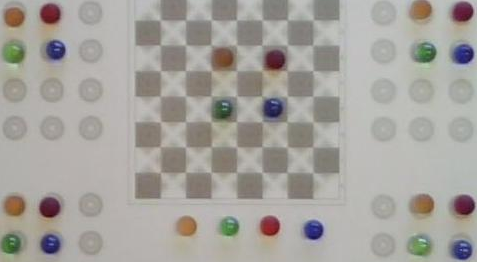
\includegraphics[width=\textwidth]{Images/Checkers-raw.png} 
\end{frame}

\begin{frame}\frametitle{Сегментация изображения}
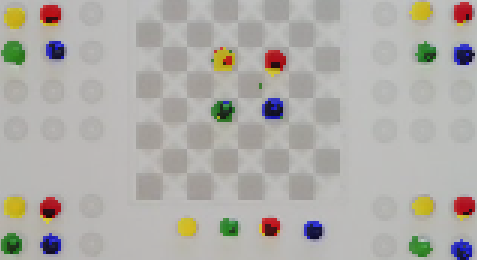
\includegraphics[width=\textwidth]{Images/Checkers-segmented.png} 
\end{frame}

\begin{frame}\frametitle{Красный канал}
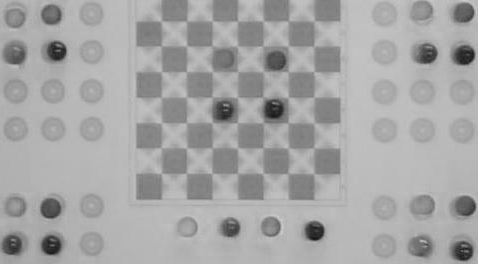
\includegraphics[width=\textwidth]{Images/Checkers-channel.png} 
\end{frame}

\begin{frame}\frametitle{RBG и HSL}
\begin{columns}
 \column{0.5\textwidth}
  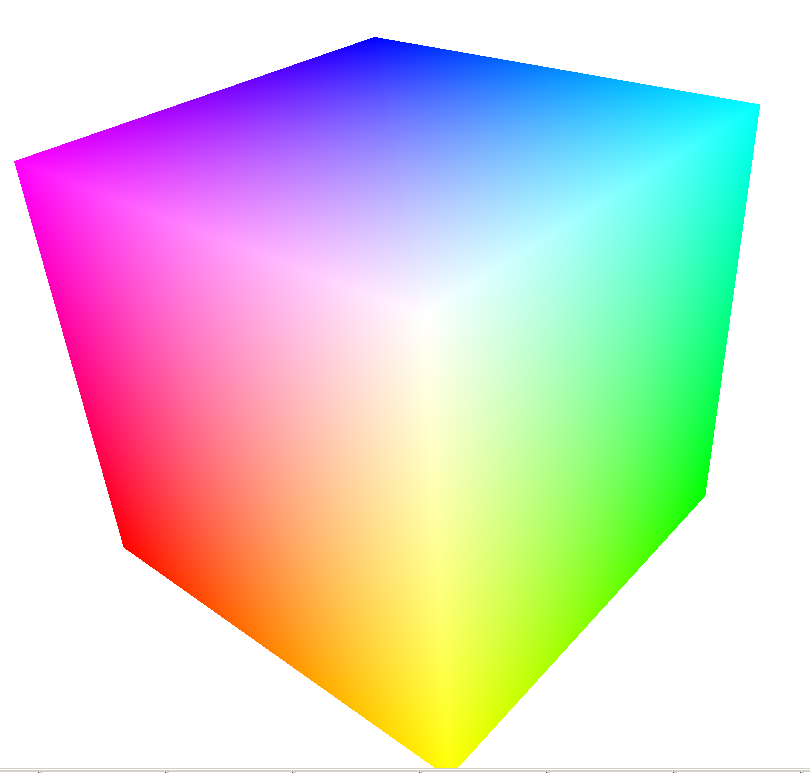
\includegraphics[width=\textwidth]{Images/RGB.png} 
 \column{0.5\textwidth}
  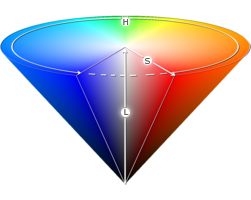
\includegraphics[width=\textwidth]{Images/HSL.jpg} 
\end{columns}
\end{frame}

\begin{frame}\frametitle{Яркость}
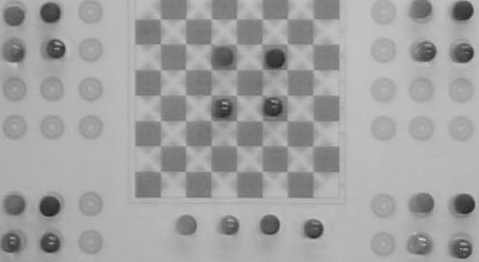
\includegraphics[width=\textwidth]{Images/Checkers-light.png} 
\end{frame}

\begin{frame}\frametitle{Насыщенность}

\includegraphics[width=\textwidth]{Images/Checkers-sat.png} 
\end{frame}

\begin{frame}\frametitle{Палитра}
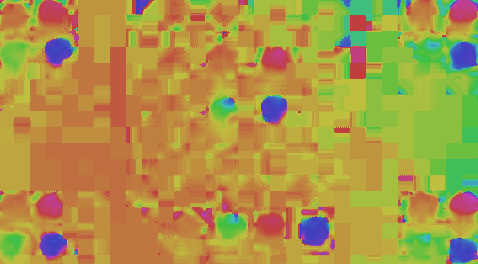
\includegraphics[width=\textwidth]{Images/Checkers-hue.png} 
\end{frame}

\begin{frame}[t]\frametitle{Функция XOR}
\begin{columns}[T]
\column{0.5\textwidth}
$$
\begin{array}{c c | c}
x_1 & x_2 & x_1\oplus x_2 \\
\hline
-1 & -1 & -1 \\
-1 & 1 & 1 \\
1 & -1 & 1 \\
1 & 1 & -1 \\
\end{array}
$$\\[1cm]

\begin{center}
\begin{tikzpicture}[y=1.5cm, x=1.5cm]
\draw[->] (-1.2,0) -- (1.4,0) node[below]{$x_1$};
\draw[->] (0,-1.2) -- (0,1.4) node[left]{$x_2$};
\draw[fill=black] (-1,-1) circle(3pt);
\draw[fill=white] (-1,1) circle(3pt);
\draw[fill=white] (1,-1) circle(3pt);
\draw[fill=black] (1,1) circle(3pt);
\end{tikzpicture}
\end{center}

\column{0.5\textwidth}
$$
(x_1,x_2) \rightarrow x_1x_2
$$\\[1cm]

$$
\begin{array}{c c | c}
x_1 & x_2 & x_1 x_2 \\
\hline
-1 & -1 & 1 \\
-1 & 1 & -1 \\
1 & -1 & -1 \\
1 & 1 & 1 \\
\end{array}
$$\\[1cm]

\begin{center}
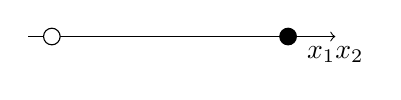
\begin{tikzpicture}[x=1.5cm,y=1.5cm]
\draw[->] (-1.2,0) -- (1.4,0) node[below] {$x_1x_2$};
\draw[fill=black] (1,0) circle(3pt);
\draw[fill=white] (-1,0) circle(3pt);
\end{tikzpicture}
\end{center}

\end{columns}
\end{frame}

\begin{frame}\frametitle{РБФ-нейрон}

$$
\begin{array}{c c}
 \uncover<1->{$Обычный нейрон$:} &  \uncover<4->{$РБФ-нейрон$:} \\
 \uncover<1->{X\rightarrow f(W\cdot X)} & \uncover<4->{X\rightarrow g(||W-X||)} \\[0.1cm]
\uncover<2->{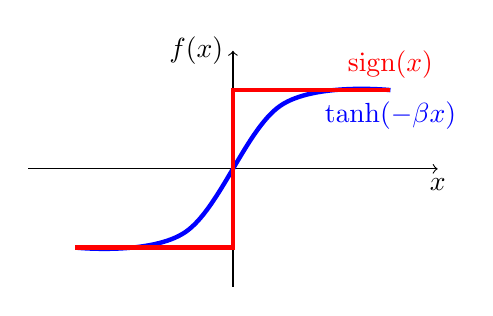
\begin{tikzpicture}[x=2cm,y=1cm]
\draw[->] (-1.3,0) -- (1.3,0) node[below] {$x$};
\draw[->] (0,-1.5) -- (0,1.5) node[left] {$f(x)$};
\draw[ultra thick,blue,smooth,tension=0.6] plot coordinates {(-1,-1) (-0.3,-0.8) (0.3,0.8) (1,1) } node[below] {${\rm tanh}(-\beta x)$};
\draw[ultra thick,red] plot coordinates {(-1,-1) (0,-1) (0,1) (1,1) } node[above] {${\rm sign}(x)$};
\end{tikzpicture}}
&
\uncover<5->{
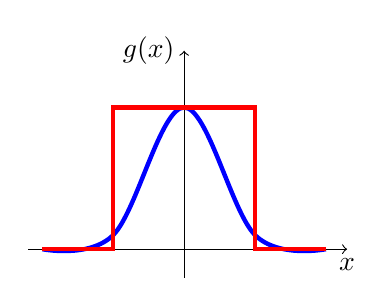
\begin{tikzpicture}[x=0.9cm,y=1.8cm]
\draw[->] (-2.2,0) -- (2.3,0) node[below] {$x$};
\draw[->] (0,-0.2) -- (0,1.4) node[left] {$g(x)$};
\draw[ultra thick,blue,smooth,tension=0.6] plot coordinates { (-2,0) (-1,0.1) (0,1) (1,0.1) (2,0) };
\draw[ultra thick,red] plot coordinates {(-2,0) (-1,0) (-1,1) (1,1) (1,0) (2,0) };
\end{tikzpicture}} \\[0.1cm]
\uncover<3->{
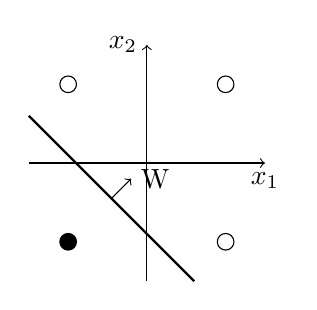
\begin{tikzpicture}[y=1cm, x=1cm]
\draw[->] (-1.5,0) -- (1.5,0) node[below]{$x_1$};
\draw[->] (0,-1.5) -- (0,1.5) node[left]{$x_2$};
\draw[fill=black] (-1,-1) circle(3pt);
\draw[fill=white] (-1,1) circle(3pt);
\draw[fill=white] (1,-1) circle(3pt);
\draw[fill=white] (1,1) circle(3pt);
\draw[thick] (-1.5,0.6) -- (0.6,-1.5);
\draw[->] (-0.45,-0.45) -- (-0.2,-0.2) node[right] {W};
\end{tikzpicture}} &
\uncover<6->{
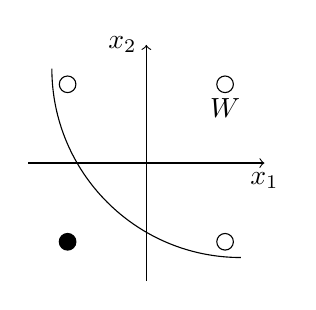
\begin{tikzpicture}[y=1cm, x=1cm]
\draw[->] (-1.5,0) -- (1.5,0) node[below]{$x_1$};
\draw[->] (0,-1.5) -- (0,1.5) node[left]{$x_2$};
\draw[fill=black] (-1,-1) circle(3pt);
\draw[fill=white] (-1,1) circle(3pt);
\draw[fill=white] (1,-1) circle(3pt);
\draw[fill=white] (1,1) circle(3pt);
\draw(-1.2,1.2) arc (180:270:2.4);
\node at (1,0.7) {$W$};
\end{tikzpicture}}\\
\end{array}
$$
\end{frame}

\begin{frame}\frametitle{Сегментация с РБФ-сетями}
$$
\begin{array}{l l}
 \mathfrak{R} = & \{R_1,R_2,R_3\} \\
 \mathfrak{G} = & \{G_1,G_2,G_3\} \\
 \mathfrak{B} = & \{B_1,B_2,B_3\} \\
\end{array}
$$


\begin{center}


\usetikzlibrary{calc,shapes}
\begin{tikzpicture}[x=2cm, y=-0.7cm]


\node (input) at (0,0) {$X$};

\node[draw=blue,ellipse] (res-1) at (4,3) {$\neg r\wedge \neg g\wedge b$};
\node[draw=blue,ellipse] (res-2) at (4,0) {$\neg r\wedge g\wedge \neg b$};
\node[draw=blue,ellipse] (res-3)at (4,-3) {$r\wedge \neg g\wedge \neg b$};

\foreach \c/\yc in {R/-1,G/0,B/1}
{
  \node[draw=blue,ellipse] (and-\c) at ($(2,\yc*3)$) {$\wedge$};
  \foreach \n in {1,2,3}
    {
    \node[draw=green,ellipse,inner sep=0.05cm] (\c-\n) at ($(1,\yc*3+\n-2)$) { $\c_\n$};
    \draw[->] (input) -- (\c-\n);
    \draw[->] (\c-\n) -- (and-\c);
    \draw[->] (and-\c) -- (res-\n);
    \draw[->] (res-\n) -- ($(res-\n.east)+(0.5,0)$);
    }
}
\end{tikzpicture}


\end{center}


\end{frame}


\end{document}